\renewcommand\thetable{\arabic{chapter}-\arabic{table}}
%\renewcommand\thefigure{\arabic{chapter}-\arabic{figure}}
\renewcommand{\theequation}{\arabic{chapter}-\arabic{equation}}
\chapter{校舍耐震資料庫}
\label{cha:database} 

學校是人才培育的場所,也是緊急災難時,居民避難的主要地方,但台灣地區學校建築在每次大地震來襲時卻常常損壞非常嚴重,尤其是老舊校舍,因興建年代久遠,其設計所依據之規範較為老舊,耐震能力可能遠低於現今結構耐震安全上之要求,有鑒於此,教育部委託了國震中心執行了「加速國中小老舊校舍及相關設備補強整建計畫」及「加速高中職及國中小老舊校舍及相關設備補強整建計畫」等計畫,進行全國學校校舍之耐震能力評估與補強研究,這些計畫建立了校舍結構物的耐震能力評估補強機制及施行的流程與細節,並且已經對全國學校校舍耐震能力作了全面性的普查,篩選出耐震能力有疑慮之校舍,並儘速透過補強或拆除新建的手段來提昇校舍的耐震能力。而此計畫進行期間所產生之資料,均收集到一「校舍耐震資料庫」中,此一資料庫為國震中心為了校舍耐震能力補強作業相關計畫所設計並建置的,收集的資料包括了典型、非典型校舍,耐震能力補強計畫中不同階段的各種相關資料。

\section{典型校舍與非典型校舍}

我國之校舍建築有極大比例在校舍的結構形式、幾何尺寸等都有相似的結構,其平面配置多如圖~\ref{fig:TSB}~所示,這類校舍都為一字型的長形建築,教室一間接著一間排列,教室外有走廊,走廊外多有柱,且樓層數不超過五樓,這一種常見的校舍在教育部的耐震能力補強計畫中統稱為「典型校舍」,典型校舍在受到地震力作用時且造成破壞,破壞的樓層通常都在一樓,而且是沿著一字形的長邊的方向破壞。由於典型校舍通常的破壞模式為沿著校舍的長向破壞,也就是走廊的方向,因此側推分析所施加的側力也就是沿著長向施加,而長向也被稱為~X~向,另外一個方向,也就一字形較短的那一邊,則是~Y~向。
%,而施加力量的方向則是正向,和力量相反的方向則是反向。

\begin{figure}[hbtp]
  \begin{center}
    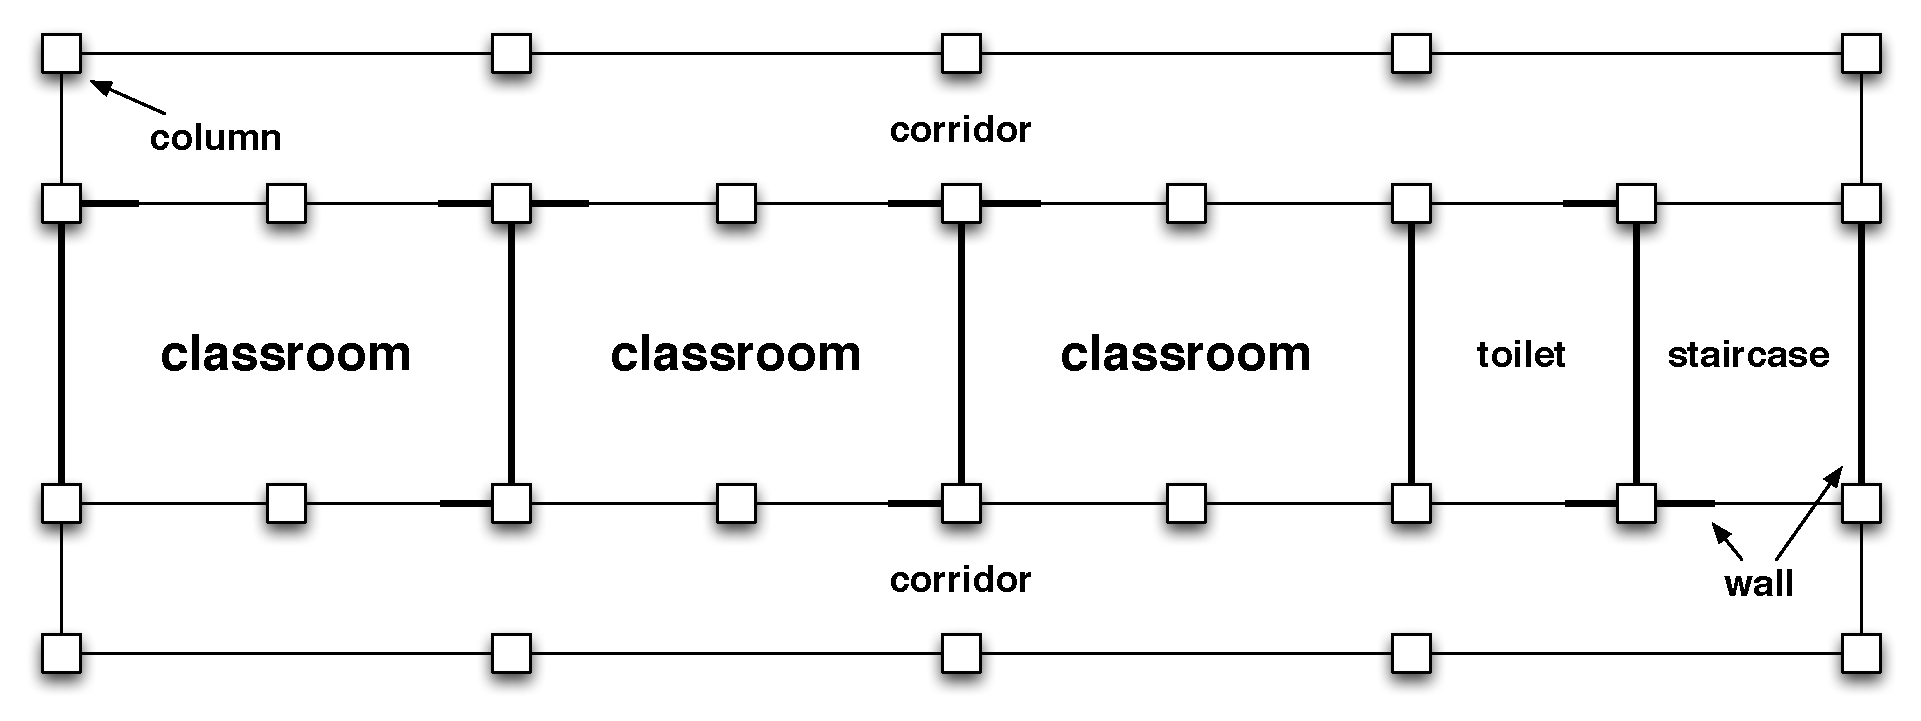
\includegraphics[width=1.0\textwidth]{figures/trad-school-building.pdf}
    \caption{典型校舍} 
    \label{fig:TSB}
  \end{center}
\end{figure}

典型校舍因為其結構形式單純,只需要少量的屬性便可以完整的描述建築物的結構,不用完整詳細的記錄所有的樑柱等構件之個別尺寸、強度與位置,只需要紀錄少量的資訊就可以建立出分析用的數值模型,因屬性數量較少,其校舍資料很適合進行各種資料分析的研究,其數量在本國所有校舍當中所佔比例也相當高,而不符合典型校舍特性之校舍,則都歸類為非典型校舍,非典型校舍可能為形狀特殊或是結構規模較大,無法只用少量的資訊就還原出該校舍之結構的數值模型,因此評估的過程非常仰賴評估人員之專業能力,而校舍耐震資料庫對於非典型校舍則主要在記錄結構物兩個主要方向的主要構件的尺寸、分佈、數量等資訊,無法詳實的反映出其特殊的設計,也因此本研究之資料探勘均針對典型校舍進行資料挖掘。

\section{資料收集範圍}

校舍的耐震能力補強流程如圖~\ref{fig:FLOW}~所示。可以分為四個大步驟,分別是校舍普查、初步評估、詳細評估、補強設計與施工,校舍普查主要之目的為全國所有校舍之基本資料建檔,並簡單調查一些主要的設計參數,是由國震中心主導進行,其性質類似於人口普查,是整個計畫中非常重要的基礎建設;接著第二個步驟的初步評估則是根據於校舍普查之基礎,對校舍進行初步評估(preliminary evaluation),其方法是基於結構物之設計及現況填寫評估表,所填寫資料再依評估公式計算出結構物耐震能力之評分等級或指數,此類方法之評估速度快,但是結果可靠度較低,主要的目的是對大量結構物之耐震能力作排序與篩選,這類型評估方法所使用之評估表與評估公式通常是使用已經收集的其他結構物資訊,用數值統計的方法迴歸,或是根據基本的結構耐震能力供需比以及專業人士相關的經驗設計得到的,其所適用之結構物類型也有所限制,評估表並不能套用到各種類型的結構物上;接著經過初步評估後,對於耐震能力有疑慮之校舍,需要進一步進行詳細評估(detailed evaluation),此類方法為對結構物進行詳細的結構耐震分析,通常是使用結構分析程式以電腦數值模擬結構物遇到地震時的非線性行為,並根據模擬結果為依據,準確詳細的檢驗評估出結構物的耐震能力;詳細評估之後,才根據技師的專業判斷,對於耐震能力堪慮之校舍,依嚴重程度,由工程專業人員,進行結構耐震能力補強之詳細評估,倘尚符合補強之經濟效益,即進一步補強其耐震能力之設計,若不符合補強之經濟效益,則將之列為拆除重建。


\begin{figure}[hbtp]
  \begin{center}
    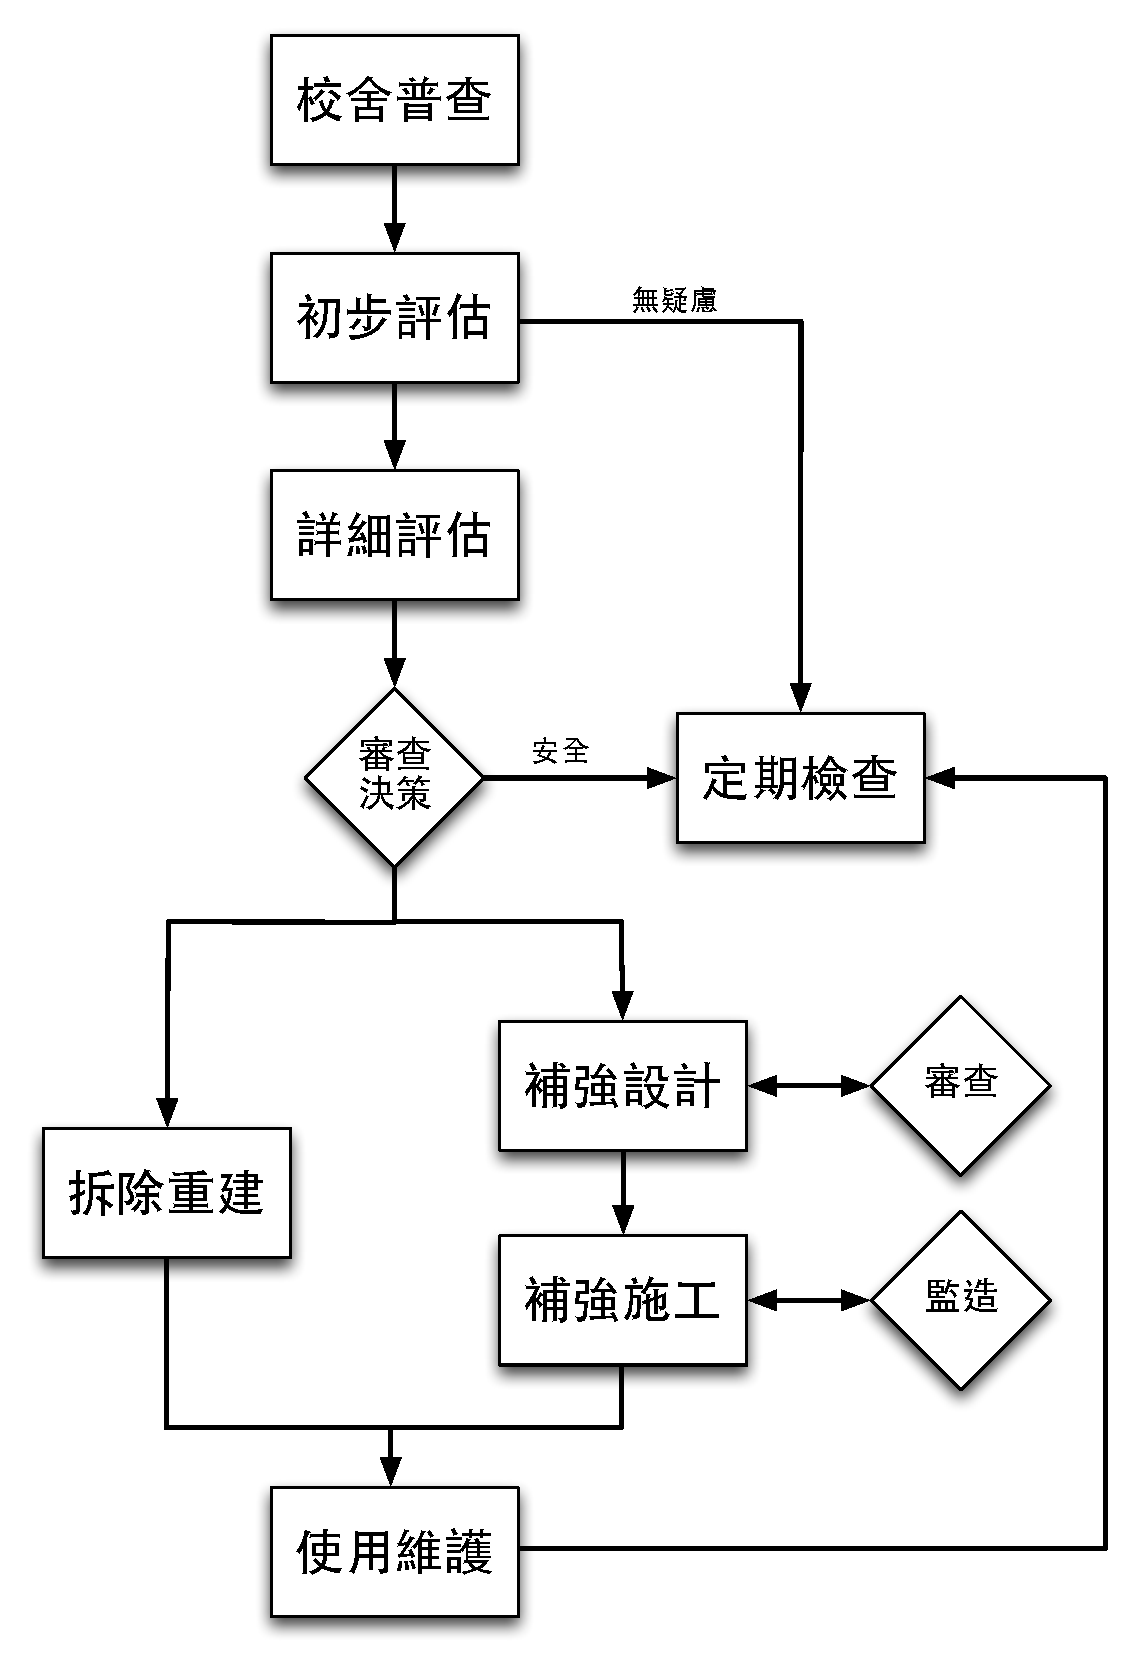
\includegraphics[width=0.8\textwidth]{figures/survey-flow.pdf}
    \caption{評估流程} 
    \label{fig:FLOW}
  \end{center}
\end{figure}

詳細評估方法的可靠度較高,但是花費相當昂貴,所需要的時間也比使用評估表要來的久很多,由於中小學校舍數量龐大,若直接大量投入人力物力,可能造成大量之資源浪費,也無法快速的鎖定耐震能力不足之校舍建築,為求有效達成此一校舍耐震評估標準需求以及基於上述標準耐震評估程序之精神,國震中心才提出先經由初步評估方法進行篩選的分段式評估方法,將校舍照其結構之耐震能力排序,以縮小問題之規模,提升整體校舍耐震能力評估作業的效率。

在此過程中會產生的校舍資料最重要的為:初步評估、詳細評估、補強設計、補強工程等四組資料,以下分別介紹四組資料之背景原理及所收集的資訊。

\subsection{初步評估}

詳細評估的原理是分別求取結構物對於地震的需求(demand)和可以承受地震的能力(capacity),然後取其比值,也就是耐震需求比(Capacity Demant Ratio,$CDR$),如果耐震需求比大於~1~則表示建築物的耐震能力足夠,足以承受未來可能發生的大地震。而初步評估雖然是簡化的評估方法,但其原理也和詳細評估相同,是以求得結構物的耐震需求以及耐震能力的比值為目標,其中,耐震需求的部分,是以校舍所在地所可能發生的~475~年週期之最大地震力作為其所需夠能夠承受之地震。至於耐震能力是根據結構物的載重元件尺寸例如牆、柱之斷面積,以及國震中心歸納之公式所推算得到之乘載元件等效強度,求得之值即為校舍之基本耐震性能~$E$,其公式為:

  \begin{equation}E = \dfrac{ 0.354 NF \times (T_{AC} \times T_{AW}) }{(-1 + 6 NF) \times (0.4 S_{aD}) \times Af} \end{equation} 

其中,~$NF$~為樓層數、$T_{AC}$~為柱等效強度、$T_{AW}$~為牆等效強度、$Af$~為總樓地板面積、$S_{aD}$~為一般工址或近斷層區域之工址設計水平譜加速度係數。
求得~$E$~後,還要根據校舍現況及專業人士判斷做調整,調整的方法則是使用國震中心先歸納整理出的調整因子~\cite{ncree03049},總共有六項:

\begin{description}
  \item[平面及立面對稱性($q_1$)]
  參考建築耐震設計規範之規定,若結構及其側向力抵抗系統的平面幾何形狀具有凹角,超過凹角部分於兩水平方向之結構 尺寸同時大於沿該方向結構總長之~15\%~以上者,表示該結構具有凹角性,則耐震能力折減為~0.95~倍;若該結構具有凹角,但超過凹角部分於任一方向之結構尺寸不足沿該方向結構總長之~15\%~,且無其他平面及立面不規則之情況,則耐震能力不予折減;若該結構不具任何凹角,且無其他平面及立面不規則之情況,則耐震能力增加為~1.05~倍。
  \item[軟弱層顯著性($q_2$)]
  若結構物之一樓因為使用性等考量,而使得二樓以上~RC~牆或磚牆於一樓中斷,致使一樓之極限層剪力強度與勁度降低,將造成地震力作用時變形集中,以致於韌性用盡,建築物就發生軟弱層破壞。故本表格依據牆體中斷的程度折減其對應之耐震能力,若~2/3~以上牆體中斷,則耐震能力折減為~0.8~倍;若~1/3~至~2/3~之牆體中斷,則耐震能力折減為~0.9~倍;若~1/3~以下之牆體中斷,則不折減其耐震能力。
  \item[裂縫鏽蝕滲水等程度($q_3$)]
  鋼筋混凝土構材若具有裂縫,代表混凝土品質不良或強度不足;保護層不足等因素使得鋼筋鏽蝕膨脹,鋼筋鏽蝕將會降低構材之強度,鋼筋鏽蝕膨脹亦會導致混凝土剝落,並加速鋼筋鏽蝕的程度,這些因素都會影響結構物的耐震安全,故以結構物整體之裂縫鏽蝕滲水等程度作為調整項目。若稍有裂縫鏽蝕滲水等情形,則耐震能力折減為~0.95~ 倍;若裂縫鏽蝕滲水等情形較為嚴重,則耐震能力折減為~0.9~倍;若無,則不折減其耐震能力。
  \item[變形程度($q_4$)]
  結構體基礎若有明顯的差異沉陷,將會造成部分構材承受額外的載重,甚至造成嚴重變形,使其耐震能力降低。故若結構體有明顯的變形程度,則耐震能力折減為~0.9~倍;若無,則不折減其耐震能力。
  \item[平面耐震性($q_5$)]
  典型的校舍建築多為數間並排相連,而呈現一字形的平面配置,其走廊形式為了滿足學生活動空間之要求,多將廊柱省略而成為懸臂走廊,故這類校舍結構系統之贅餘度較少。校舍之結構系統贅餘度越多,則於地震時越能發揮韌性與力量重分配的能力,將有助於減少地震時倒塌之可能性,故本研究將典型的校舍建築簡單分為三大類,一為廊外無柱或其他,其耐震能力不予調整;一為單走廊且廊外有柱或中間走廊,其結構系統無懸臂走廊之形式且贅餘度較多,故其耐震能力增加為~1.1~倍;最後一種為雙走廊且廊外有柱,其結構系統贅餘度最多,故其耐震能力增加為~1.2~倍。
  \item[短柱嚴重性($q_6$)]
  一般老舊校舍之柱箍筋間距多為~20cm~至~30cm~左右,其剪力強度不高,且老舊校舍於設計時假設為純梁柱系統,並沒有考慮教室窗台及樓梯廁所等牆壁開氣窗所造成之短柱效應,然而這種短柱效應將會使得剪力容量不足之柱於地震時發生非預期之剪力破壞,導致結構韌性不足,若該校舍有過多之柱受到短柱效應之影響,將易造成校舍瞬間倒塌。故若校舍因窗台或氣窗造成短柱現象之柱根數達到全部柱根數之~50\%~以上,則耐震能力折減為~0.9~倍,若不足~50\%~則不予折減其耐震能力。值得注意的是,短柱嚴重性具有方向性,故評估時只需考慮評估方向之短柱比率是否超過一半即可,另一方向開窗等因素造成之短柱效應不需考慮。
\end{description}


最後乘上調整因子後得到之耐震指標為~$Is$~,其公式如下:

  \begin{equation}Is = E \times \prod_{i=1}^6 q_i \end{equation} 

%  \begin{equation}Is = E \times q1 \times q2 \times q3 \times q4 \times q5 \times q6 \end{equation} 

$Is$~是一個百分制系統,以~80~作為耐震能力堪慮之標準,若校舍調查所得之耐震指標~$Is$~值低於~80~分,表示其耐震能力頗為不足,確有耐震疑慮,若有相當於~475~年週期發生一次之最大地震時,將有嚴重損壞或倒塌之疑慮,應最優先進行耐震能力之補強設計與施工;耐震指標~$Is$~值介於~80~分及~100~分,表示校舍耐震性之安全係數尚不符合耐震設計規範對於此等重要性建築物之耐震需求,仍有耐震性能不足之疑慮,若有相當於~475~年週期發生一次的最大地震時,將有可能發生嚴重結構上之破壞,其耐震能力之提升列為次優先對象;耐震指標~$Is$~值高於~100~分,表示其尚無耐震能力不足之疑慮,若有相當於~475~年週期發生一次之最大地震時,應不至於發生嚴重結構上之破壞。雖然根據上述耐震指標~$Is$~低於~100~分就須接受耐震能力補強,但根據觀察校舍資料內資料,初步評估結果~90~至~100~分進行詳細評估後,絕大部分都不須進行補強,80~分以下~70~分以上也有一些進行詳細評估後也是裁定不需補強,因此雖然耐震指標~$Is$~不是最後決定補強之最後依據,但也具有相當之影響力。

%初步評估相較於詳細評估的模擬運算而言,是簡化許多的耐震能力評估方式,評估的方式是使用地震中心根據過往資料與相關規範所設計而得,其設計的基礎與詳細評估的 $CDR$ 值相同,皆為校舍的耐震能力與耐震需求的比值,主要的對象為典型校舍,假設校舍之破壞位置為長向的一樓,耐震需求為則為建築物需要能承受其所在地所可能發生的的475年週期最大地震之地震力,由推估的校舍載重以及地震之地表加速度推估而得。而耐震能力則是根據校舍之柱、牆等尺寸,並根據實驗數據推估所得到的等效強度,兩者相除後再乘上調查人員根據校舍現況所填入之調整參數 $Q$,所得到的 $Is$ 即為使用初步評估表格所評估之校舍耐震能力。

\subsection{詳細評估}

美國針對鋼筋混凝土(RC)建築物之耐震能力規範~ATC-40\cite{applied1996seismic}~中,建議用來評估建築物耐震能力之方法稱為容量震譜法(capacity spectrum method),此一評估方法可以分為兩個部分,第一部分是進行側推分析(pushover analysis)取得容量震譜(capacity spectrum),流程如圖~\ref{fig:capacity-curve}~所示,第二部分是根據建築物所在地的各種相關資訊和規範取得需求震譜(demand spectrum),接著使用容量震譜法(capacity spectrum method)以取得建築物性能點,根據性能點座標帶入公式計算可以得到建築物的破壞地表加速度以及耐震能力指標(aseismic ability index),如圖~\ref{fig:performance-point}~所示。

\begin{figure}[hbtp]
  \begin{center}
    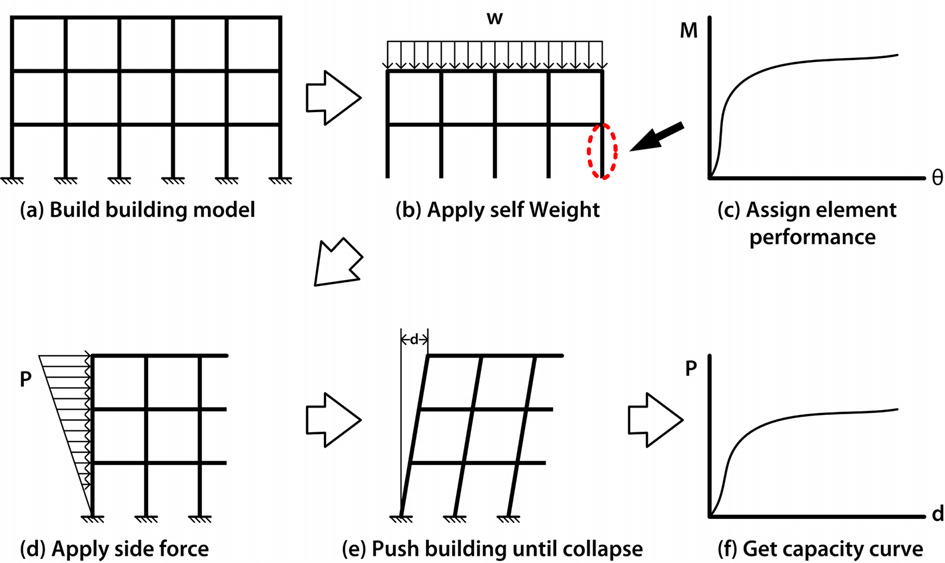
\includegraphics[width=1.0\textwidth]{figures/capacity-curve.png}
    \caption{結構物容量震譜計算流程圖}
    \label{fig:capacity-curve}
  \end{center}
\end{figure}

求取容量震譜的側推分析法需要先建立建築物完整的非線性分析模型,此模型要由進行評估的專業人士根據建築物的幾何尺寸資訊來建立基本的建築物框架。接著根據建築物的材質計算建築物自身重量以及需要承載的人員和配設物件之重量,並將其附加到柱、牆等承載元件上。接著最重要的是設定建築物各構成元件如樑、柱、牆受力時的非線性行為,這些力與變形的關係多為實驗得到或是利用其他分析模擬方法得到的。至此,側推分析要用的數值模型才算建立完成。而側推分析其程序是依照~FEMA-440\cite{fema440}~
之建議,逐步地給結構模型施加增量的側向外力,將結構物向某一方向推動,每次增量即進行一次結構分析計算每一構件之應力與變位,之後與上一次的分析結果累加即可得到每一個構件於此受力階段之反應,並判斷構件是否破壞,例如開裂、降伏,甚至達到極限強度,之後各構件依其破壞程度更新其行為,例如改變其勁度,或者將已發生破壞的構件從結構模型中抽離,如此重複分析直到結構不穩定而崩垮為止,側推分析完成後可以得到建築物之容量震譜。

需求震譜是根據建築物環境現況,參考規範製成之地震需求頻譜。參考的環境狀況如土層種類,堅硬的土層可以讓建築物有較好的抗震能力。另外靠近斷層的建築物在地震發生時往往會因為斷層於地震時產生的反應而受到嚴重的損害,因此建築物與斷層的距離也納入參考的資料之一,稱為近斷層效應(special effects of near-source earthquakes),其他還需要的資料有地層資料、地震震區等,綜合這些資料並參考規範即可得到該建築物所需符合之需求震譜。

\begin{figure}[hbtp]
  \begin{center}
    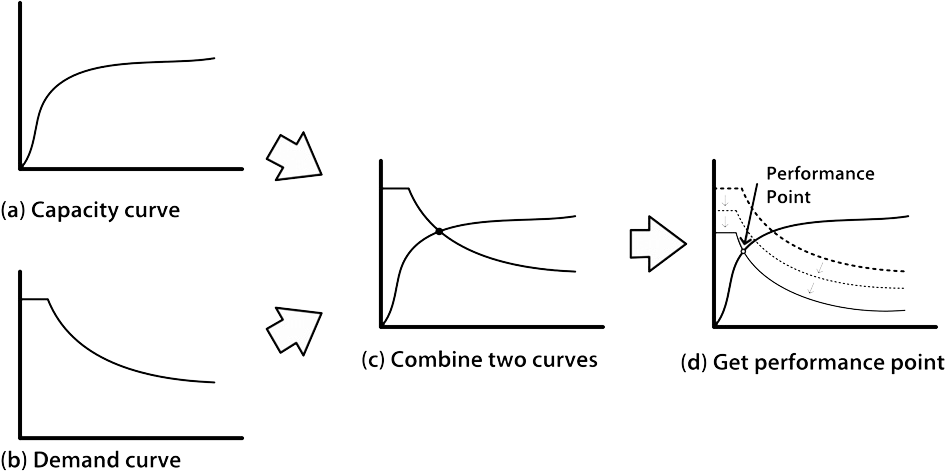
\includegraphics[width=1.0\textwidth]{figures/performance-point.png}
    \caption{結構物性能點計算流程圖}
    \label{fig:performance-point}
  \end{center}
\end{figure}

容量震譜法(capacity spectrum method)最後是將需求震譜以及容量震譜轉換格式後相疊,求取建築物之性能點(performance point),性能點之物理意義為該建築物在特定水準地震下所能承受之最大變位及剪力,但是由於結構物受地震力作用進入非線性行為時,結構物的阻尼效應會產生消能的作用,因此還要視情況對需求曲線進行折減,此為一個迭帶運算的過程,可能需要不斷折減需求曲線,並進行性能點正確性的檢核,直到檢核通過,才能得到建築物真正之性能點如圖~\ref{fig:performance-point}~,由建築物性能點之座標帶入公式可以求得建築物的破壞地表加速度(collapse ground acceleration,~$A_C$),詳細評估所使用的耐震能力值為耐震需求比($CDR$),其定義如下:

\begin{equation} CDR = \dfrac{A_C}{A_D} \label{eq:CDR}\end{equation} 

$A_D$~為根據建築物所在地的並依據規範所得到的,建築物所需要能承受的~475~年週期最大地震所產生之地表加速度,$CDR$~大於~1~代表此一棟建築物能夠承受該地區~475~年一遇的最大地震。

\subsection{補強設計與竣工資料}

如果校舍經過詳細評估過後,負責的專業人士認為此棟校舍確實有安全疑慮,但尚可以補強,不需要拆除重建時,則該棟校舍就會進入補強設計階段,此一階段的工作也是委託專業人士執行,負責的專業人士需要依據詳細評估的結果,設計出兩種不同的補強方案,並且對不同的補強方案進行詳細的耐震能力評估,因此這個階段的資料包括兩組補強設計的資料,以及兩組補強後的耐震能力詳細評估資料。補強設計收集的資料主要為使用的補強工法以及補強量,主要收集的補強工法包括了六類:增設構件、柱補強、牆補強、樑補強、減載措施、基礎補強。

增設構件所可能增加的構件包括了剪力牆、翼牆、斜撐、柱、樑等,皆為結構物之乘載構件,其優點是可以有效且直接的增加結構物的乘載能力,缺點是增加的構件可能讓結構物的隔間變化,讓使用功能性變差。而另外一種補強方式則是在現有的構件上加強,包括了柱補強、牆補強、樑補強,這三種補強工法都是針對現有的結構元件加強,例如擴柱、鋼板貼片、複合材料貼片等,這類方法不改變節結構之基本設計,對於結構物之使用性影響較小,但仍然可能影響到建築物之採光、通風等。減載則是屬於比較消極的補強方式,藉由減少結構物的乘載重量來檢少結構物受到地震力作用而倒塌的可能性,而其措施包括了拆除樓層,通常為從上往下拆除、樓層數則是專業人士評估判斷,另一種方式則是變更用途,如果校舍結構物對於自重本身的乘載能力已經足夠,則可以考慮改變部分樓層的用途,減少其所需要乘載的載重,而減載措施相較於其它幾種補強方式,是屬於成本較低的補強方式。

補強設計階段,負責設計的專業人士會提出不同的補強方案做為校舍補強工程的參考,而後根據預算和學校單位的需求以及校舍安全性等因素綜合考量以決定補強方案,並進行補強工程,在工程完成後,國震中心還會收集相關的資料,包括補強方法、補強構件的數量、不同類型工程之花費、補強材料強度報告等,而在這些資料當中,補強工程的經費是一個非常重要的數據,因為此一資料數值是校舍補強流程當中最後一個階段才會得到的,但卻是在整個校舍補強計畫當中,初期編列預算就非常需要,影響很大的數據。

\section{資料庫結構}

此一校舍耐震資料庫使用的是用途非常廣泛的關連式資料庫,其實體關係圖如圖~\ref{fig:school-er}~所示,實體關係圖是在初步設計資料庫結構時所用,可以呈現關連式資料庫中各資料表間的關係,使用的呈現方式是實體關聯模型(ER model),此一資料模型是透過實體(entity)與關係(relation)兩種物件來作表示,實體是所欲儲存資料於現實中之實際物體,關係則是各實體間的關係,設計之結果可以用實體關係圖之形式表示,實體關係圖則以矩形代表實體、菱形代表關係、橢圓形代表實體的屬性。


\begin{figure}[hbtp]
  \begin{center}
    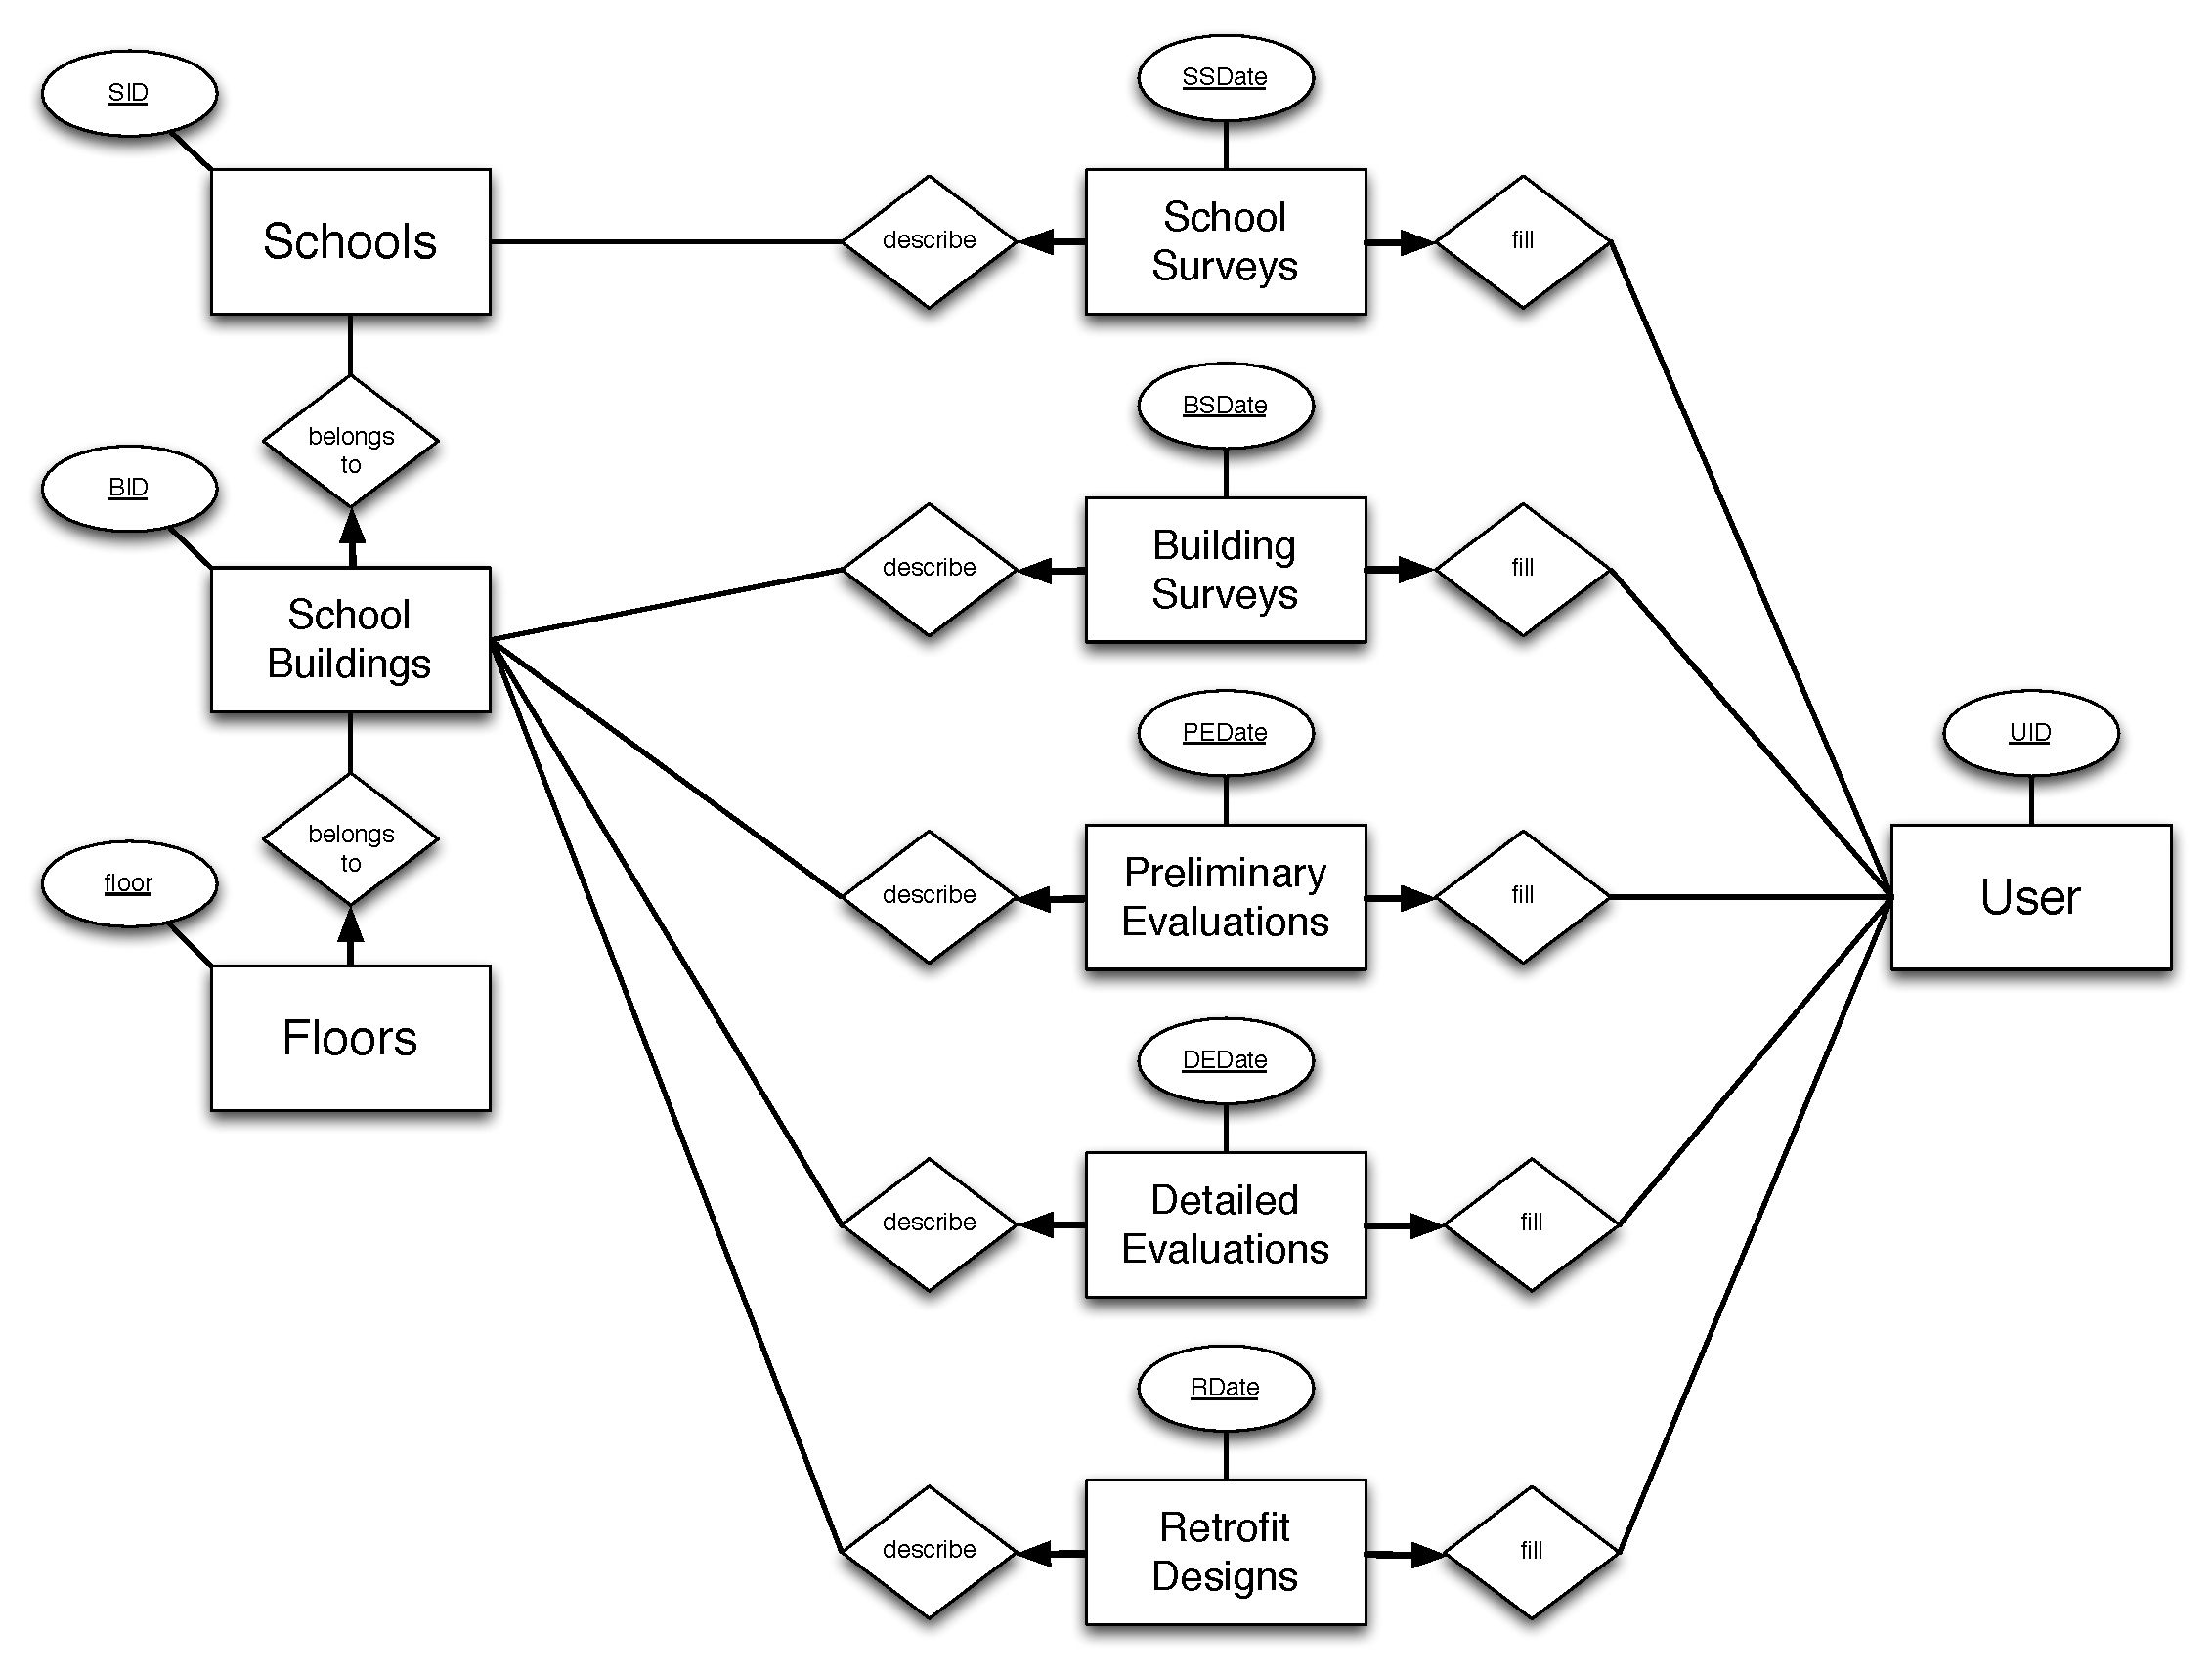
\includegraphics[width=1.0\textwidth]{figures/school-er.pdf}
    \caption{校舍耐震資料庫實體關係圖} 
    \label{fig:school-er}
  \end{center}
\end{figure}


圖~\ref{fig:school-er}~之標示採簡化之表示法,即各表格之屬性(attribute)只標示出其主鍵(primary key),校舍耐震資料庫的基礎是~School~和~School Building~兩個資料表,Schools~代表所有學校基本資料集合之實體組(entity set),構成~Schools~之每個實體(entity)均是代表某學校,資料庫系統是以紀錄了此學校的基本資料,包含學校名稱、地址、GPS~座標等資訊為屬性,而~School Buildings~代表所有校舍集合之實體組,構成~School Buildings~之每個實體均是代表某學校之某校舍,每棟校舍是以紀錄其校舍名稱、建造年代、設計圖等資訊為屬性,因每一間學校內多有多棟校舍,故其與~Schools~間為一對多之關係,而校舍的樓層數為不定數量,故把樓層相關之資料屬性獨立出來存放在~Floors~資料表,其代表所有樓層集合之實體組,構成~Floors~之每個實體均是代表某學校某校舍之某一樓層,每層樓是以儲存該樓層之樓高、樓地板面積、教室間數這類各樓層獨有之資訊,由於每一棟校舍會有多層樓,故其與~School Buildings~為一對多之關係。

有了以上的基礎後,資料庫設計便基於圖~\ref{fig:FLOW}~之流程,將不同階段的調查表、評估分為不同之資料表。圖中之~School Surveys~方塊即代表所有校舍普查集合之實體組;構成~School Surveys~之每個實體均是代表對某學校所作之某次簡普查,每次調查是以紀錄學校整體之損害狀況等調查資料為屬性代表之,由於某學校之狀況會隨時間改變,學校之調查會定期重新調查,故其與~Schools~間為一對多之關係,此假設同一日不會有兩次的調查,故其與~School Surveys~不另設獨有的~ID~為主鍵,而是採~SID(調查學校)與~SSDATE(調查日期)之組合;構成~Building Surveys~之每個實體均是代表對某學校之某校舍所作之某次校舍普查,其即以該次調查所填調查表格之資料為屬性代表之;構成~Preliminary Evaluations~之每個實體均是代表對某學校之某校舍所作之某次初步評估,其即以該次評估所填評估表格之資料為屬性代表之,表格之詳細內容則為\nameref*{appendix-pe}所記載之資訊;Detailed Evaluations~實體組代表詳細評估之集合,表格之詳細內容則為\nameref*{appendix-de}所記載之資訊;Retrofit Designs~實體組則是補強設計之集合,表格之詳細內容則為\nameref*{appendix-re}所記載之資訊,而後續包括補強施工和竣工報告等都與~School Buildings~實體有一樣的關聯設計。這些調查表之實體組與校舍間如同~School Surveys~與~Schools~間之關係,由於每棟校舍均可能於不同時間進行不只一次,故其與~School Building~間關係為一對多關係。Users~實體組代表所有填表人之集合,系統是以紀錄某填表人之簡易資料,包括姓名、聯絡方法、職稱等為屬性代表之,因為一個填表人可能負責評估多間校舍,故~Users~與上述代表評估調查之實體組間之~fill~關係組也為一對多之關係。







